\documentclass[14pt,a4paper]{extarticle}
% =============================================================
% preamble.tex — общая преамбула отчётов по дисциплине
% «Стили и методы программирования. Часть 2»
% Оформление по СТП БГУИР 01-2024; сборка XeTeX (tectonic)
% =============================================================

% Encoding and language
\usepackage{fontspec}
\usepackage[russian]{babel}

% Times New Roman font
\setmainfont{Times New Roman}
\setmonofont{Menlo}[Scale=0.85]

% Page geometry: STP 2.1.1
\usepackage{geometry}
\geometry{left=30mm, right=15mm, top=20mm, bottom=20mm}

% Line spacing: STP 2.1.1
\usepackage{setspace}
\singlespacing

% Allow TeX a bit more flexibility to avoid overflow
\pretolerance=1000
\tolerance=2000
\emergencystretch=3em

% Paragraph indent
\usepackage{indentfirst}
\setlength{\parindent}{1.25cm}

% Page numbers
\usepackage{fancyhdr}
\pagestyle{fancy}
\fancyhf{}
\fancyfoot[R]{\thepage}
\renewcommand{\headrulewidth}{0pt}
\fancypagestyle{plain}{%
  \fancyhf{}%
  \fancyfoot[R]{\thepage}%
  \renewcommand{\headrulewidth}{0pt}%
}

% Math
\usepackage{amsmath,amssymb}

% Graphics
\usepackage{graphicx}
\usepackage{float}
\usepackage{xcolor}

% Tables
\usepackage{booktabs}
\usepackage{tabularx}
\usepackage{multirow}
\usepackage{longtable}

% Captions
\usepackage{caption}
\captionsetup[figure]{
  labelsep=endash,
  justification=centering,
  font={normalsize},
  name=Рисунок
}
\captionsetup[table]{
  labelsep=endash,
  justification=raggedright,
  singlelinecheck=false,
  font={normalsize},
  name=Таблица
}

% Section formatting
\usepackage{titlesec}
% Каждый раздел с новой страницы. \newpage внутри \titleformat срабатывает
% после записи в оглавление и сбивает номера страниц, поэтому \clearpage
% ставится перед самой командой \section.
\usepackage{etoolbox}
\pretocmd{\section}{\clearpage}{}{}
\titleformat{\section}
  {\normalfont\fontsize{14}{18}\selectfont\bfseries}
  {\thesection}{0.5em}{\MakeUppercase}
\titlespacing*{\section}{1.25cm}{0pt}{14pt}

\titleformat{\subsection}
  {\normalfont\fontsize{14}{18}\selectfont\bfseries}
  {\thesubsection}{0.5em}{}
\titlespacing*{\subsection}{1.25cm}{14pt}{14pt}

\titleformat{\subsubsection}
  {\normalfont\fontsize{14}{18}\selectfont\bfseries}
  {\thesubsubsection}{0.5em}{}
\titlespacing*{\subsubsection}{1.25cm}{14pt}{14pt}

% Unnumbered sections
\newcommand{\sectioncenter}[1]{%
  \newpage
  \phantomsection
  \addcontentsline{toc}{section}{#1}
  \begin{center}
    \textbf{\MakeUppercase{#1}}
  \end{center}
  \vspace{14pt}
}

% Table of contents formatting
\usepackage{tocloft}
\renewcommand{\cftsecfont}{\normalfont}
\renewcommand{\cftsecpagefont}{\normalfont}
\renewcommand{\cftsubsecfont}{\normalfont}
\renewcommand{\cftsubsecpagefont}{\normalfont}
\renewcommand{\cftsecleader}{\cftdotfill{\cftdotsep}}
\renewcommand{\cftdotsep}{1}
% babel переопределяет \contentsname при \begin{document}, поэтому через captionsrussian
\addto\captionsrussian{\renewcommand{\contentsname}{СОДЕРЖАНИЕ}}
\renewcommand{\cfttoctitlefont}{\hfill\normalfont\bfseries}
\renewcommand{\cftaftertoctitle}{\hfill}

% Lists
\usepackage{enumitem}
\setlist[itemize]{noitemsep, topsep=0pt, leftmargin=1.25cm, label=--}
\setlist[enumerate]{noitemsep, topsep=0pt, leftmargin=1.25cm}

% Code listings: fvextra корректно работает с Unicode под XeTeX
% (listings переставляет символы «», —, № в комментариях)
\usepackage{fvextra}
\fvset{
  frame=single,
  fontsize=\small,
  numbers=left,
  numbersep=6pt,
  breaklines=true,
}
\newcommand{\code}[1]{\texttt{#1}}

% Hyperlinks
\usepackage{hyperref}
\hypersetup{
  colorlinks=true,
  linkcolor=black,
  urlcolor=blue,
  citecolor=black,
}

% Number figures and tables within sections
\numberwithin{figure}{section}
\numberwithin{table}{section}
\numberwithin{equation}{section}

% Титульный лист: \makelabtitle{номер}{тема}{дата}
\newcommand{\makelabtitle}[3]{%
  \begin{titlepage}
  \thispagestyle{empty}
  \begin{center}

  МИНИСТЕРСТВО ОБРАЗОВАНИЯ РЕСПУБЛИКИ БЕЛАРУСЬ

  \vspace{0.5em}

  Учреждение образования

  \vspace{0.5em}

  \textbf{<<Белорусский государственный университет информатики и радиоэлектроники>>}

  \vspace{2em}

  Факультет компьютерных систем и сетей

  \vspace{0.5em}

  Кафедра программного обеспечения информационных технологий

  \end{center}

  \vspace{3em}

  \begin{center}
  \textbf{ОТЧЕТ}

  \vspace{0.5em}

  по практической работе №#1

  \vspace{0.5em}

  по дисциплине

  \vspace{0.5em}

  <<Стили и методы программирования. Часть 2 (МДН)>>

  \vspace{0.5em}

  на тему

  \vspace{0.5em}

  <<#2>>
  \end{center}

  \vspace{5em}

  \begin{flushright}
  \begin{minipage}{0.5\textwidth}
  \textbf{Выполнил:}\\
  Лебедевич Артем Владимирович\\
  магистрант 2 курса группы 556301

  \vspace{0.6em}

  \textbf{Преподаватель:}\\
  Парамонов Антон Иванович\\
  кандидат технических наук\\
  доцент

  \vspace{0.6em}

  \textbf{Дата:} #3
  \end{minipage}
  \end{flushright}

  \vfill

  \begin{center}
  Минск, 2026~г.
  \end{center}

  \end{titlepage}
}

\graphicspath{{figures/}}

\begin{document}

\makelabtitle{1}{Установка и настройка среды логического программирования Prolog}{24.09.2026}

\tableofcontents

\newpage

\section{Цель работы}

Освоить установку и настройку инструментальных средств логического программирования на примере SWI-Prolog, получить навыки работы с интерактивной средой (top-level), загрузки и выполнения простейших программ.

\section{Используемое ПО}

Параметры программной среды приведены в таблице~\ref{tab:env}.

\begin{table}[H]
\caption{Программная среда}
\label{tab:env}
\centering
\begin{tabularx}{\textwidth}{@{}lX@{}}
\toprule
Параметр & Значение \\
\midrule
Реализация Prolog & SWI-Prolog 10.0.2 (threaded, 64 bits), сборка \code{arm64-darwin} \\
Способ установки & менеджер пакетов Homebrew, формула \code{swi-prolog} (лицензия BSD-2-Clause) \\
Операционная система & macOS 26.6.2 (сборка 25G83) \\
Аппаратная платформа & Apple M4 Pro, архитектура arm64 \\
Интерпретатор & \code{/opt/homebrew/bin/swipl}, консольный top-level в терминале zsh \\
Редактор & Visual Studio Code (внешний редактор исходных файлов) \\
Просмотр исходников & PlDoc~--- встроенный веб-сервер документации SWI-Prolog \\
Рабочая директория & \code{\textasciitilde/PycharmProjects/prolog/lab\_01} \\
\bottomrule
\end{tabularx}
\end{table}

\textbf{Обоснование выбора.} SWI-Prolog~--- свободная, активно развиваемая реализация, совместимая со стандартом ISO и синтаксисом Эдинбургского Пролога, в котором написаны учебные примеры; она ставится одной командой под macOS на Apple Silicon, тогда как Visual Prolog работает только под Windows. Кроме того, SWI-Prolog содержит развитые средства отладки (трассировщик, диагностику при загрузке) и встроенную справку, что важно на этапе освоения языка.

\section{Ход выполнения работы}

\subsection{Установка и настройка}

Интерпретатор установлен из репозитория Homebrew командой \code{brew install swi-prolog}; вместе с ним установлены зависимости (\code{gmp}, \code{libarchive}, \code{openssl@3}, \code{pcre2}, \code{unixodbc} и~др.). Работоспособность проверена командами оболочки \code{which swipl} и \code{swipl --version} (рисунок~\ref{fig:install}).

\begin{figure}[H]
\centering
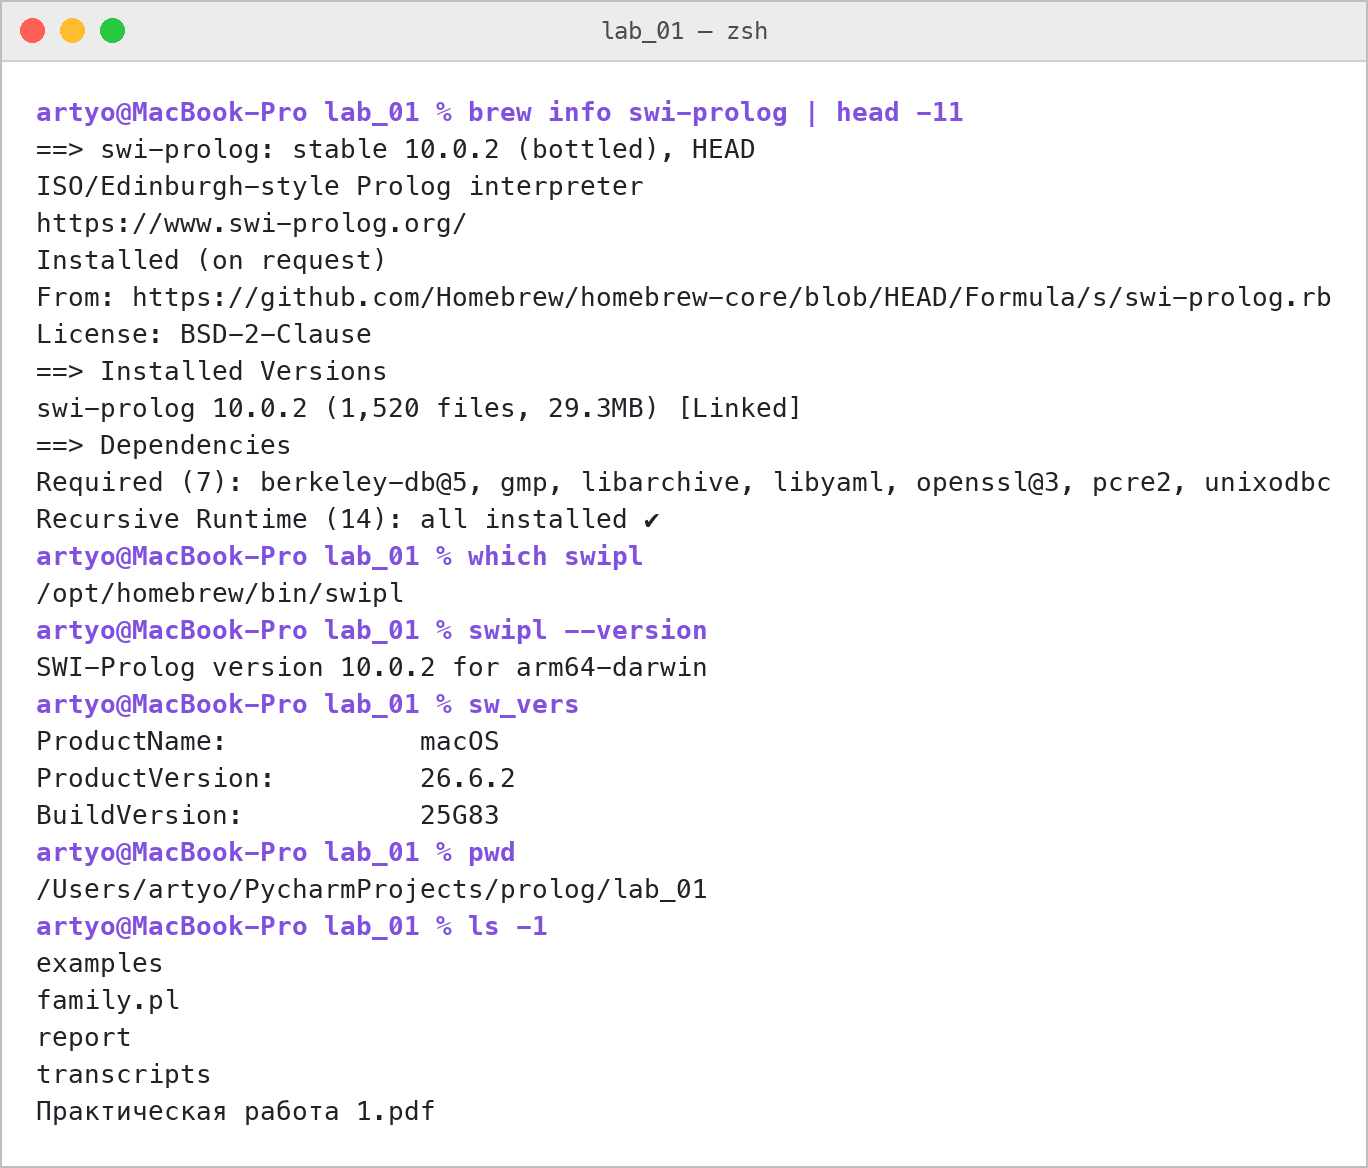
\includegraphics[width=0.85\textwidth]{fig01_install.png}
\caption{Сведения об установленном пакете, версия интерпретатора, ОС и рабочая директория}
\label{fig:install}
\end{figure}

Для файлов программ создана рабочая директория \code{lab\_01} внутри репозитория \code{prolog}. Интерпретатор запускается из неё, поэтому она становится текущей директорией Prolog, и файлы загружаются по короткому имени без пути. Текущая директория проверяется запросом \code{working\_directory(D, D)}, содержимое~--- запросом \code{ls}; при необходимости директорию меняют запросом \code{working\_directory(\_, 'путь')} или \code{cd('путь')}. Запуск интерпретатора, вывод версии и проверка рабочей директории показаны на рисунке~\ref{fig:start}. Запрос \code{version.} повторно выводит приветствие с номером версии, а флаг \code{version} хранит её в числовом виде: $100002$ соответствует версии 10.0.2.

\begin{figure}[H]
\centering
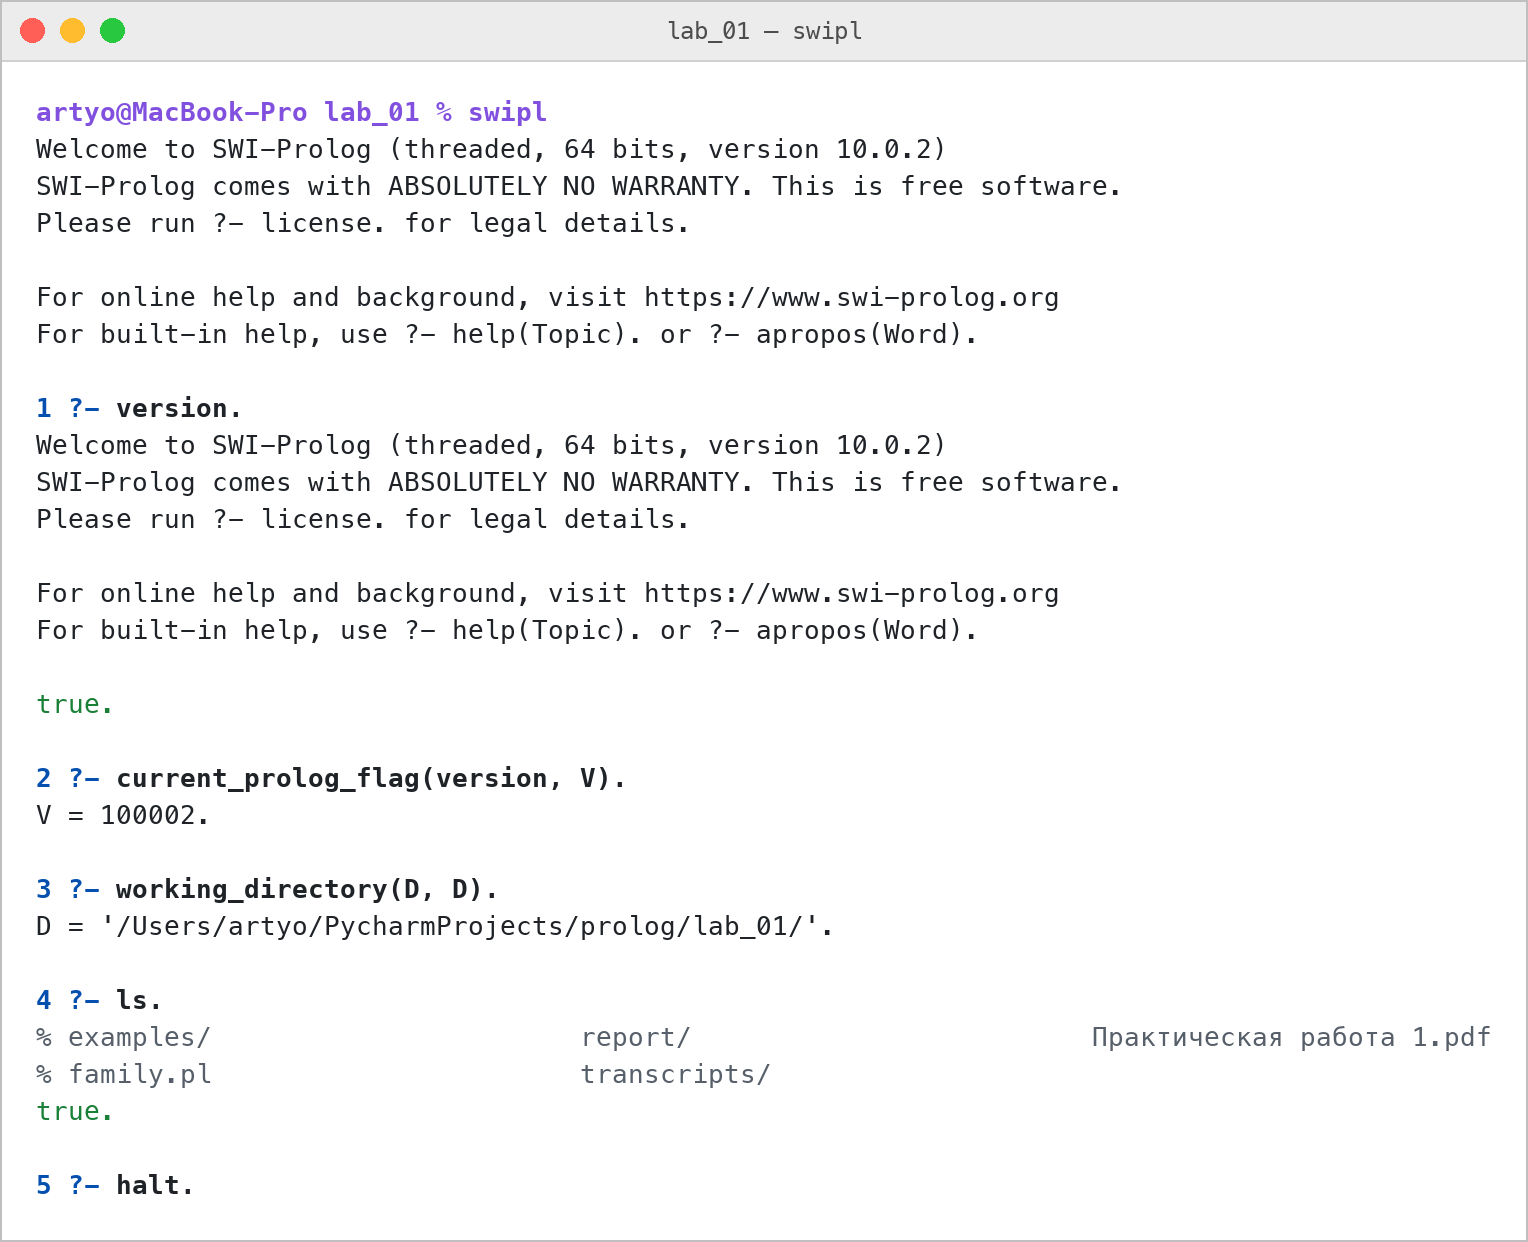
\includegraphics[width=0.95\textwidth]{fig02_start.png}
\caption{Запуск интерпретатора, запрос версии и проверка рабочей директории}
\label{fig:start}
\end{figure}

Исходные тексты редактируются во внешнем редакторе (VS Code), а из среды SWI-Prolog их удобно просматривать через PlDoc~--- встроенный веб-сервер документации. Он запускается запросом \code{doc\_server(4040)} и показывает файлы рабочей директории (рисунок~\ref{fig:pldoc-dir}) и исходный текст с подсветкой синтаксиса: головы определяемых предикатов выделены красным, переменные~--- курсивом, комментарии~--- зелёным (рисунок~\ref{fig:pldoc-src}). Встроенный редактор вызывается запросом \code{edit(family)}; какой редактор он откроет, задаёт флаг \code{editor}.

\begin{figure}[H]
\centering
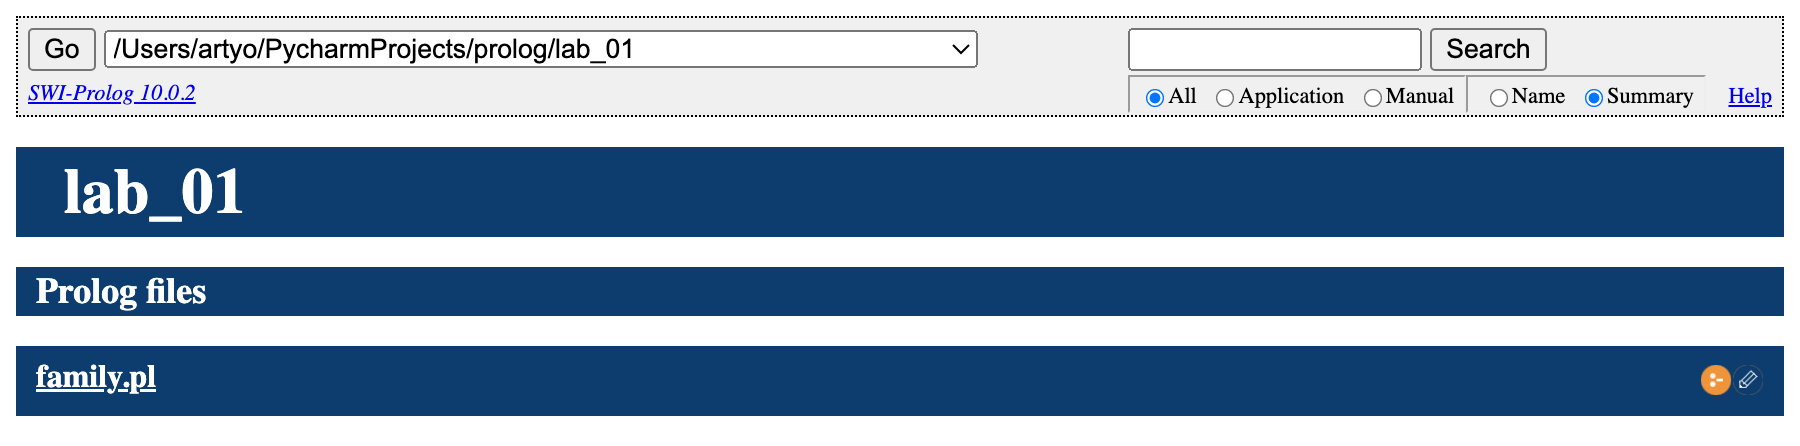
\includegraphics[width=0.9\textwidth]{fig11_pldoc_dir.png}
\caption{Рабочая директория в веб-интерфейсе PlDoc}
\label{fig:pldoc-dir}
\end{figure}

\begin{figure}[H]
\centering
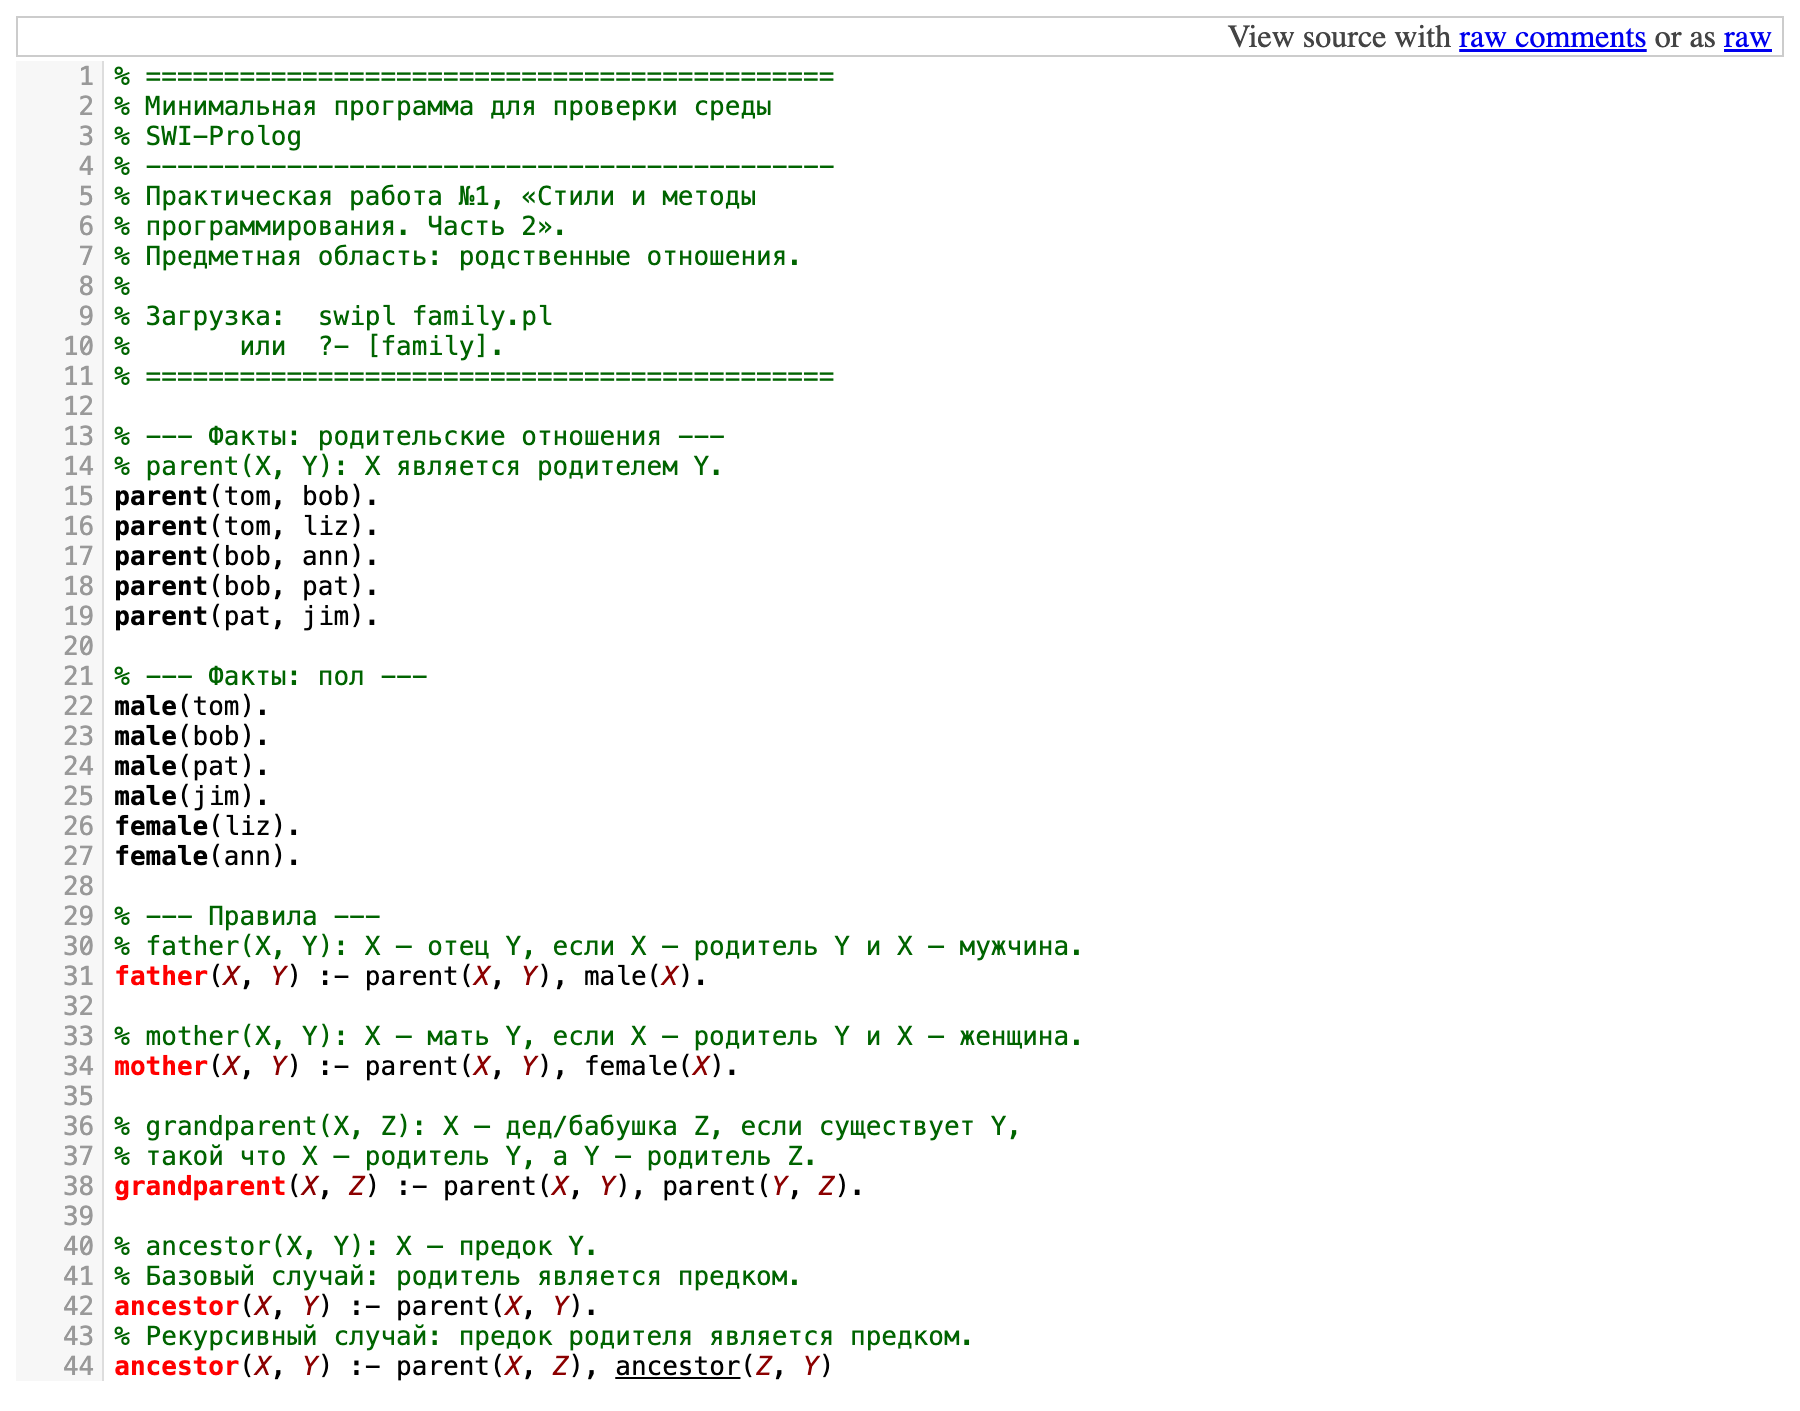
\includegraphics[width=0.8\textwidth]{fig10_pldoc_src.png}
\caption{Исходный текст программы \code{family.pl} в режиме просмотра PlDoc}
\label{fig:pldoc-src}
\end{figure}

\subsection{Освоение команд top-level}

Освоенные команды интерактивной среды перечислены в таблице~\ref{tab:commands}. Каждая команда вводится после приглашения \code{?-} и завершается точкой.

\begin{longtable}{@{}p{0.43\textwidth}p{0.53\textwidth}@{}}
\caption{Команды top-level SWI-Prolog}\label{tab:commands}\\
\toprule
Команда & Назначение \\
\midrule
\endfirsthead
\toprule
Команда & Назначение \\
\midrule
\endhead
\code{swipl family.pl} & запуск интерпретатора из оболочки с загрузкой файла \\
\code{?- [family].} & загрузка (консультация) файла \code{family.pl}; расширение \code{.pl} подставляется автоматически \\
\code{?- consult('family.pl').} & то же в явной форме; при повторной загрузке клаузы файла заменяются, а не дублируются \\
\code{?- make.} & перезагрузка всех файлов, изменённых после последней загрузки \\
\code{?- listing(ancestor/2).} & вывод клауз предиката в нормализованном виде \\
\code{?- version.} & вывод сведений о версии \\
\code{?- help(halt/0).} & справка по предикату из встроенного руководства \\
\code{?- apropos(consult).} & поиск по руководству по ключевому слову \\
\code{?- working\_directory(D, D).} & получение текущей рабочей директории \\
\code{?- ls.} & список файлов текущей директории \\
\code{?- trace.} & включение пошаговой трассировки следующего запроса \\
\code{?- notrace.} & выключение трассировки; среда остаётся в режиме отладки \code{[debug]} \\
\code{?- nodebug.} & выход из режима отладки \\
\code{?- halt.} & завершение работы интерпретатора (или Ctrl+D) \\
\code{;} & запрос следующего решения (возврат) \\
\code{Enter} или \code{.} & прекращение перебора решений \\
\bottomrule
\end{longtable}

Загрузка файла из командной строки и из top-level, а также вывод предиката командой \code{listing} показаны на рисунке~\ref{fig:consult}. Команды \code{[family].} и \code{consult('family.pl')} отвечают \code{true.}, а \code{listing/2} печатает клаузы \code{ancestor/2} с переименованными переменными и стандартными отступами.

\begin{figure}[H]
\centering
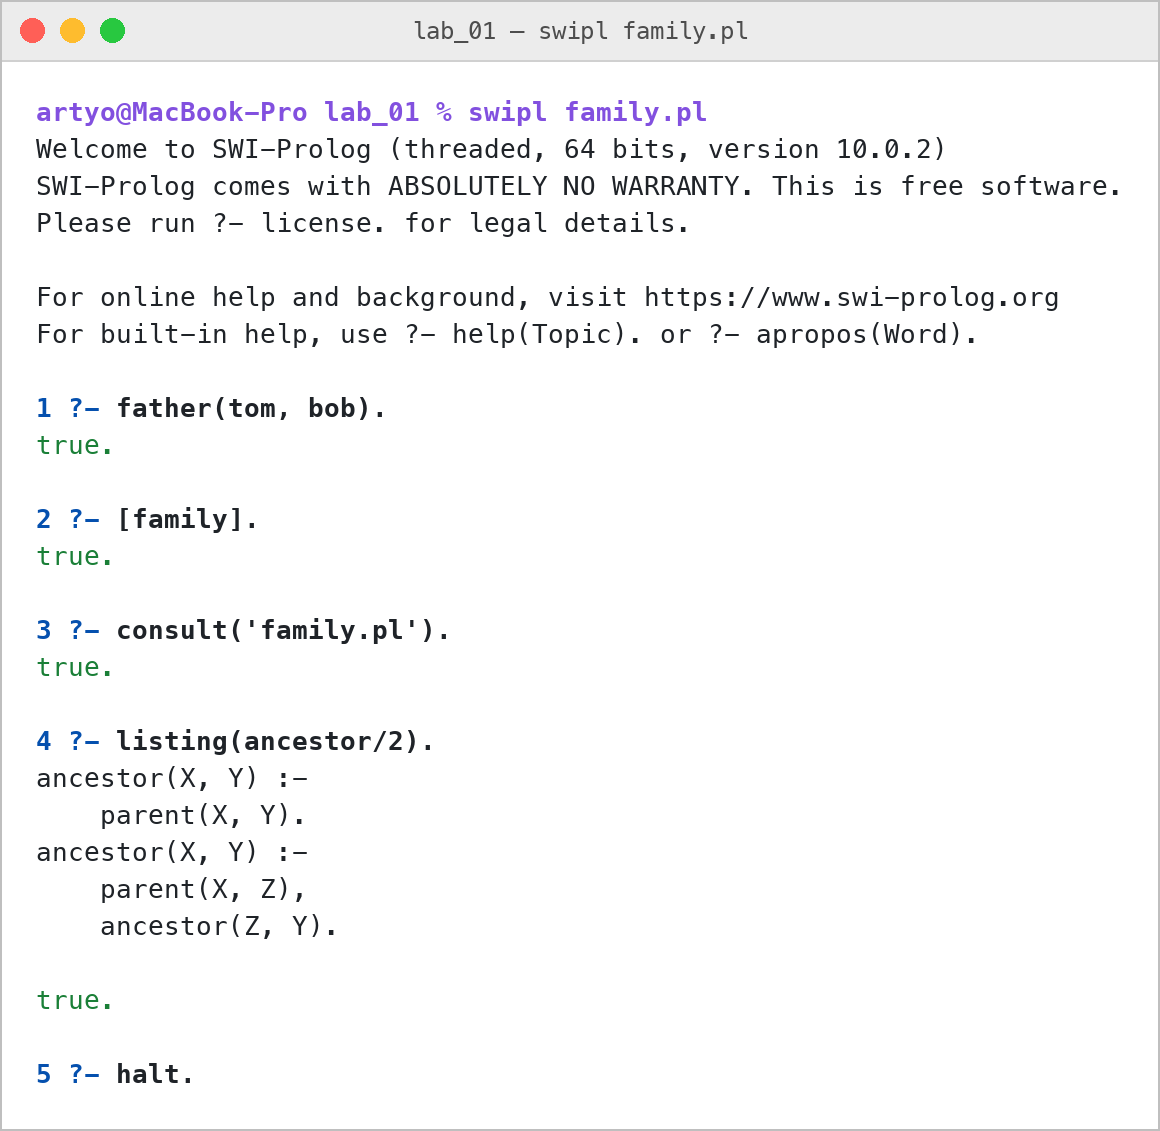
\includegraphics[width=0.75\textwidth]{fig03_consult.png}
\caption{Загрузка программы и просмотр клауз предиката}
\label{fig:consult}
\end{figure}

Встроенная справка (рисунок~\ref{fig:help}) выводится прямо в терминал. При первом вызове \code{help/1} заметна задержка в несколько секунд: система загружает индекс руководства.

\begin{figure}[H]
\centering
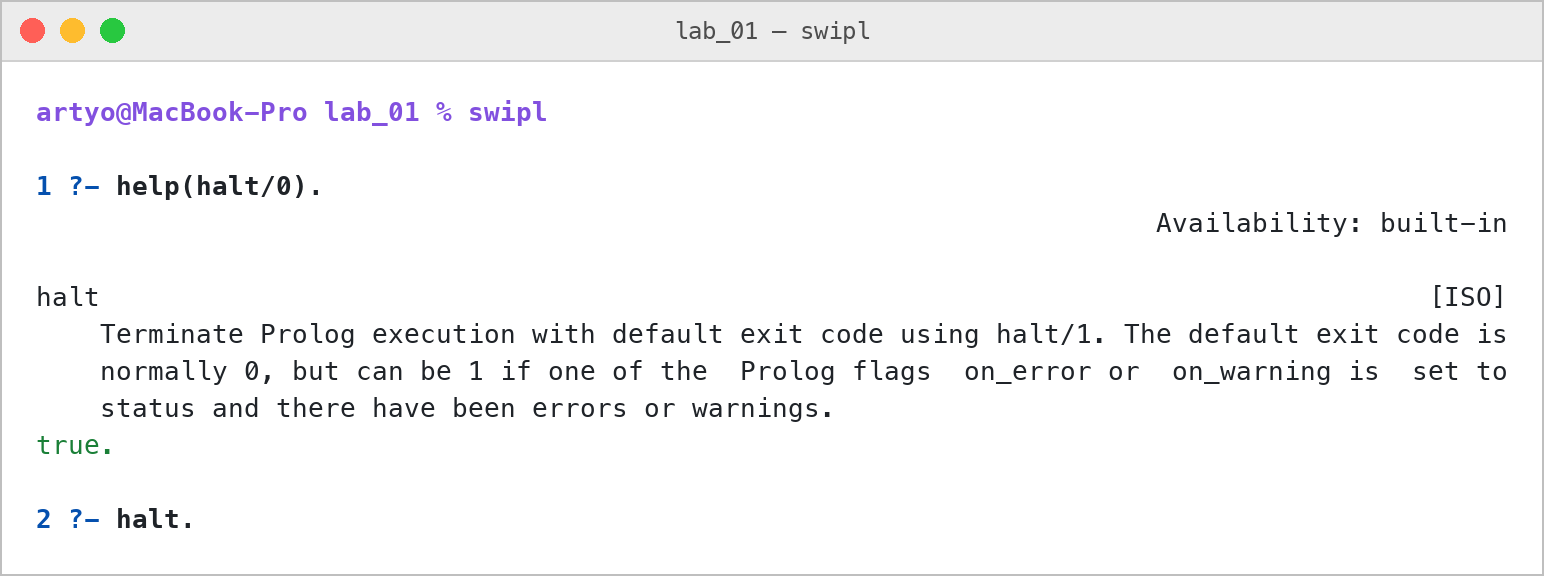
\includegraphics[width=0.95\textwidth]{fig04_help.png}
\caption{Справка по предикату \code{halt/0}}
\label{fig:help}
\end{figure}

Трассировка запроса \code{grandparent(X, jim)} приведена на рисунке~\ref{fig:trace}. Трассировщик останавливается на каждом \emph{порту} процедурной модели Бёрда: \code{Call}~--- вызов цели, \code{Exit}~--- успешный выход, \code{Fail}~--- неуспех, \code{Redo}~--- повторный вход при возврате. Нажатие \code{c} (или Enter) выполняет шаг (\code{creep}). В скобках указана глубина вложенности цели: 12~--- \code{grandparent}, 13~--- вызовы \code{parent} из его тела. Хорошо видно, как Пролог перебирает факты \code{parent(X, Y)} сверху вниз и для каждого проверяет вторую цель \code{parent(Y, jim)}: пары \code{tom--bob}, \code{tom--liz}, \code{bob--ann} отбрасываются, и только для \code{bob--pat} обе цели выполняются. После нажатия \code{;} перебор продолжается с последней точки выбора, но других решений нет, и запрос завершается ответом \code{false}.

\begin{figure}[H]
\centering
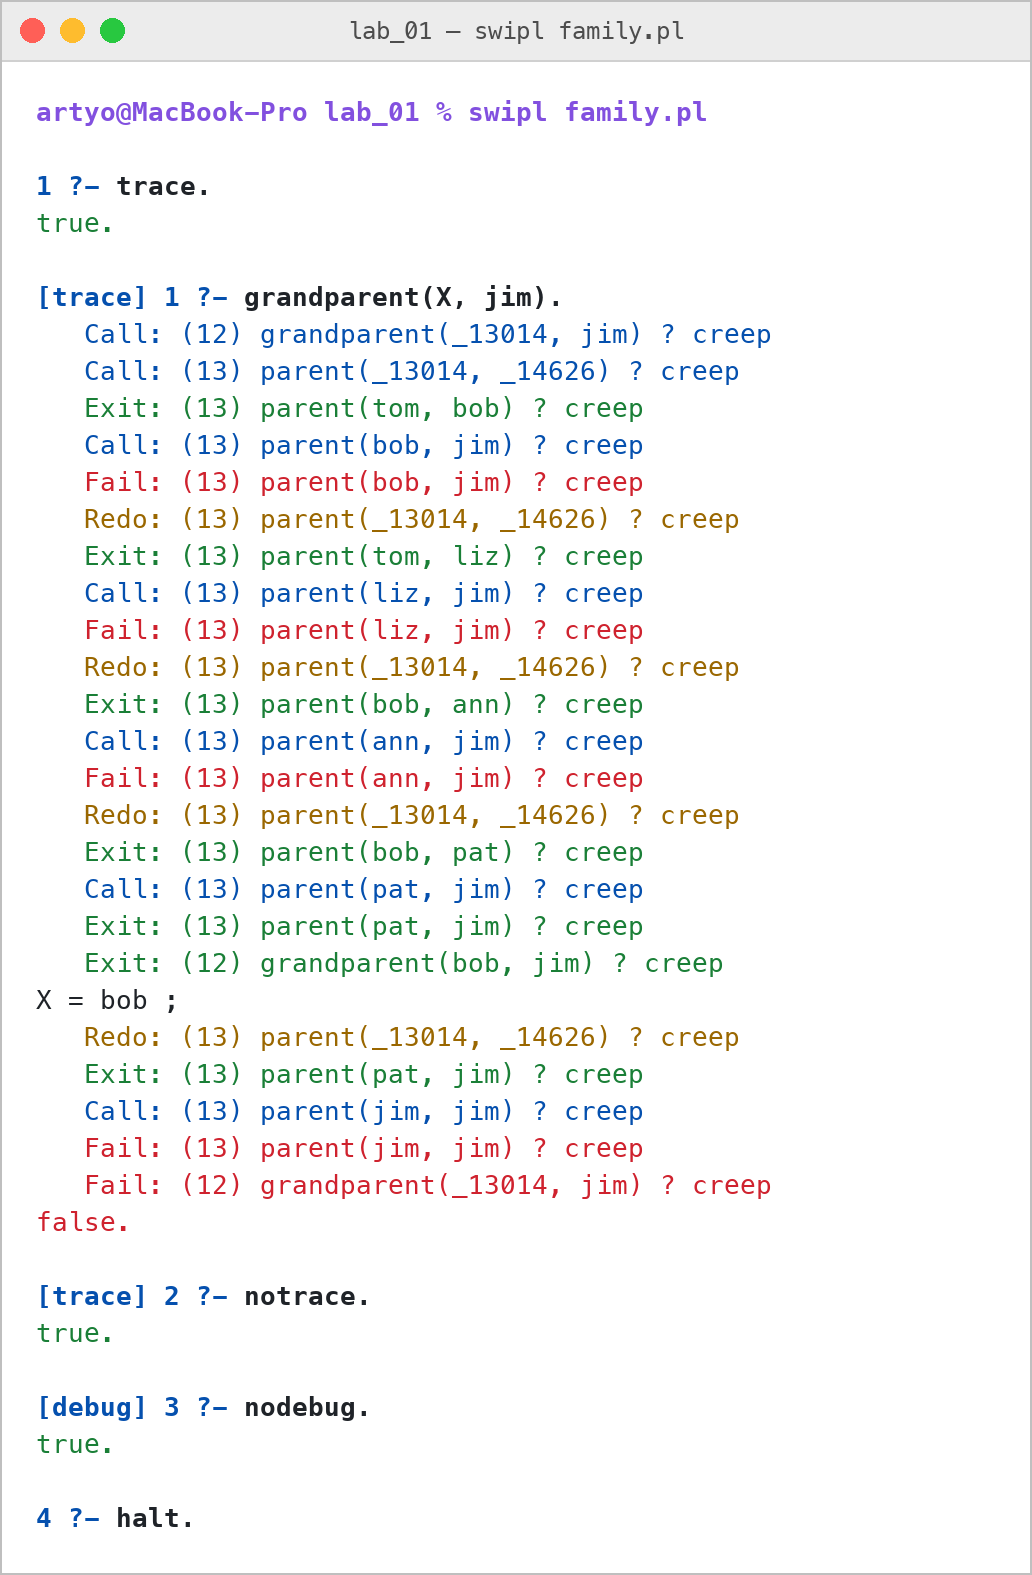
\includegraphics[width=0.7\textwidth]{fig05_trace.png}
\caption{Пошаговая трассировка запроса \code{grandparent(X, jim)}}
\label{fig:trace}
\end{figure}

\subsection{Текст программы}

Программа <<Родственные отношения>> из Приложения~1 к заданию записана в формате SWI-Prolog в файл \code{lab\_01/family.pl}. База знаний содержит пять фактов \code{parent/2}, шесть фактов о поле (\code{male/1}, \code{female/1}) и четыре правила. Правила \code{father/2} и \code{mother/2} уточняют отношение <<родитель>> полом, \code{grandparent/2} строит цепочку из двух отношений \code{parent} через общую переменную \code{Y}, а \code{ancestor/2}~--- рекурсивное правило с базовым случаем (родитель~--- предок) и рекурсивным шагом (предок родителя~--- тоже предок).

\VerbatimInput{../family.pl}

\subsection{Результаты контрольных запусков}

Все 13 запросов из Приложения~2 выполнены после загрузки программы командой \code{swipl family.pl}. Сводка результатов приведена в таблице~\ref{tab:queries}; результаты совпадают с ожидаемыми.

\begin{longtable}{@{}p{0.05\textwidth}p{0.29\textwidth}p{0.29\textwidth}p{0.28\textwidth}@{}}
\caption{Результаты контрольных запросов}\label{tab:queries}\\
\toprule
№ & Запрос & Полученный ответ & Что демонстрирует \\
\midrule
\endfirsthead
\toprule
№ & Запрос & Полученный ответ & Что демонстрирует \\
\midrule
\endhead
1 & \code{parent(tom, bob).} & \code{true.} & наличие факта \\
2 & \code{parent(bob, tom).} & \code{false.} & отсутствие факта \\
3 & \code{male(tom).} & \code{true.} & проверка факта \\
4 & \code{female(tom).} & \code{false.} & отрицательный факт \\
5 & \code{father(tom, bob).} & \code{true.} & работа правила \\
6 & \code{mother(liz, ann).} & \code{false.} & правило не выполняется \\
7 & \code{parent(tom, X).} & \code{X = bob ; X = liz.} & перебор решений \\
8 & \code{parent(X, pat).} & \code{X = bob.} & поиск родителя \\
9 & \code{grandparent(X, jim).} & \code{X = bob ; false.} & правило \code{grandparent} \\
10 & \code{ancestor(tom, X).} & \code{bob, liz, ann, pat, jim; false.} & рекурсивное правило \\
11 & \code{parent(tom, X).} + \code{;} & \code{X = bob ; X = liz.} & механизм возврата \\
12 & \code{ancestor(X, jim).} + \code{;} & \code{pat, tom, bob; false.} & поиск всех предков \\
13 & \code{parent(X, Y).} + \code{;} & пять пар \code{X-Y} & полный перебор базы \\
\bottomrule
\end{longtable}

\textbf{Проверка фактов и правил (запросы 1--6)}, рисунок~\ref{fig:basic}. Запросы без переменных~--- это вопросы <<да/нет>>. Запросы~1 и~3 совпадают с фактами базы и получают ответ \code{true}. Факта \code{parent(bob, tom)} в базе нет, а Пролог работает в предположении замкнутого мира: всё, что нельзя вывести, считается ложным, поэтому ответ~--- \code{false} (запросы~2 и~4). В запросе~5 правило \code{father} сводит цель к двум подцелям \code{parent(tom, bob)} и \code{male(tom)}, обе выполняются. В запросе~6 первая же подцель \code{parent(liz, ann)} неуспешна, так как мать \code{ann} в базе не указана.

\begin{figure}[H]
\centering
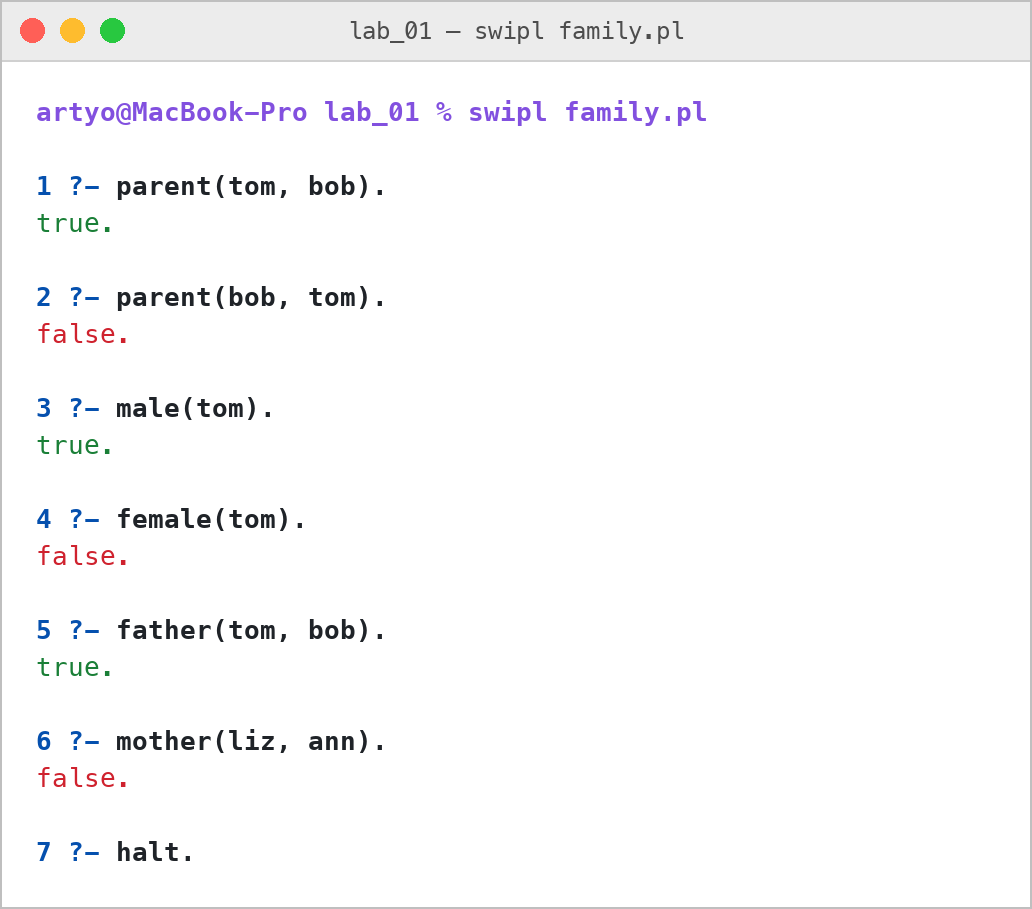
\includegraphics[width=0.62\textwidth]{fig06_basic.png}
\caption{Запросы 1--6: проверка фактов и правил}
\label{fig:basic}
\end{figure}

\textbf{Запросы с переменными (7--10)}, рисунок~\ref{fig:vars}. Пролог ищет такие значения переменных, при которых цель выводима, унифицируя запрос с головами клауз. Для \code{parent(tom, X)} подходят два факта, и после \code{;} выдаётся второе решение. В запросе~8 решение единственное, и SWI-Prolog сразу ставит точку: благодаря индексации по второму аргументу он знает, что других подходящих клауз нет. В запросе~9 найден дед \code{jim}~--- \code{bob}; после \code{;} система проверяет оставшиеся варианты и отвечает \code{false}. Запрос~10 перебирает всех потомков \code{tom}: сначала детей по нерекурсивной клаузе (\code{bob}, \code{liz}), затем более далёких потомков по рекурсивной (\code{ann}, \code{pat}, \code{jim}).

\begin{figure}[H]
\centering
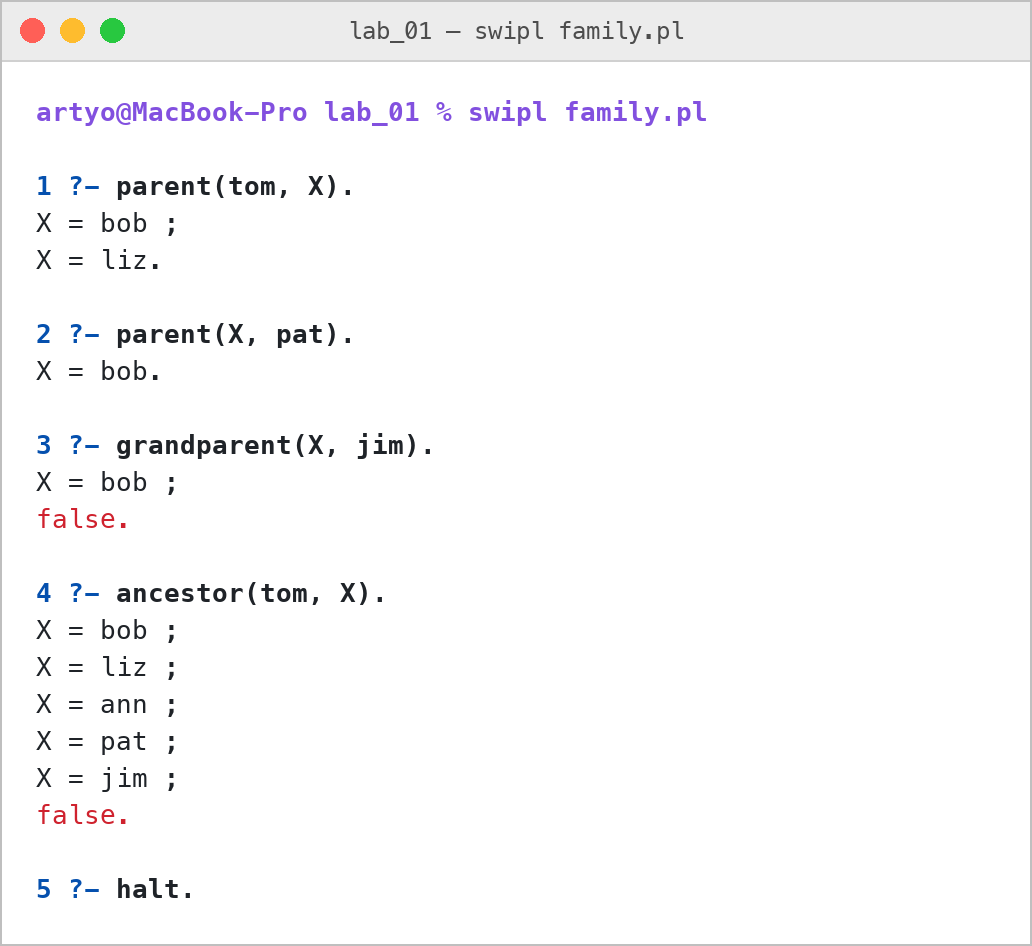
\includegraphics[width=0.62\textwidth]{fig07_variables.png}
\caption{Запросы 7--10: поиск решений}
\label{fig:vars}
\end{figure}

\textbf{Возврат (запросы 11--13)}, рисунок~\ref{fig:backtrack}. После каждого решения, если остались непроверенные альтернативы, top-level ждёт ввода: \code{;} заставляет систему вернуться к последней точке выбора и искать следующее решение. Порядок предков в запросе~12 (\code{pat}, \code{tom}, \code{bob}) определяется стратегией поиска в глубину: сначала срабатывает первая клауза \code{ancestor} (прямой родитель \code{pat}), затем рекурсивная, в которой факты \code{parent(X, Z)} перебираются в порядке записи. Запрос~13 последовательно выдаёт все пять пар базы. Дополнительно показан встроенный предикат \code{findall/3}, собирающий все решения в список без ручного нажатия \code{;}.

\begin{figure}[H]
\centering
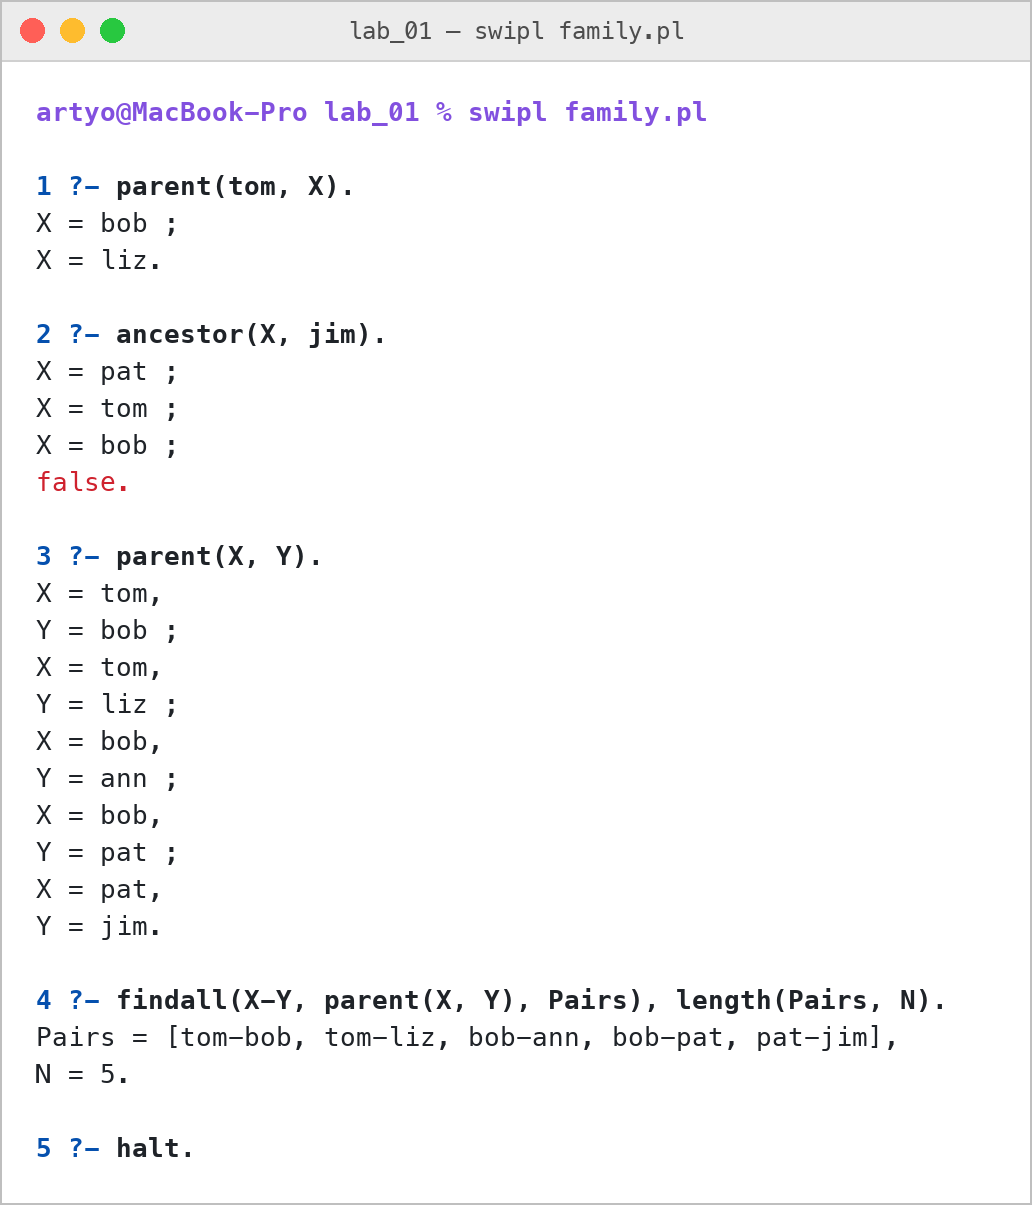
\includegraphics[width=0.62\textwidth]{fig08_backtracking.png}
\caption{Запросы 11--13: перебор решений возвратом}
\label{fig:backtrack}
\end{figure}

\section{Анализ результатов}

При работе со средой отмечены следующие особенности.

\begin{enumerate}
\item \textbf{Детерминированные и недетерминированные ответы.} SWI-Prolog завершает ответ точкой, если уверен, что других решений нет (\code{X = bob.} в запросе~8), и ждёт ввода, если осталась точка выбора (\code{X = bob} в запросе~9). Поэтому после последнего решения иногда появляется \code{false}: оно означает не ошибку, а исчерпание альтернатив. В методических указаниях для запроса~9 ожидается просто \code{X = bob}~--- это то же решение, SWI-Prolog лишь дополнительно сообщает, что больше решений нет.
\item \textbf{Представление переменных.} В трассировке несвязанные переменные выводятся как \code{\_13014}~--- внутренние имена, которые меняются от запуска к запуску.
\item \textbf{Нумерация и история запросов.} Приглашение имеет вид \code{N ?-}, где \code{N}~--- номер запроса в истории. История сохраняется отдельно для каждой рабочей директории в \code{\textasciitilde/.config/swi-prolog/dir-history}, поэтому после перезапуска нумерация продолжается.
\item \textbf{Режимы отладки.} После \code{trace.} приглашение получает префикс \code{[trace]}, после \code{notrace.}~--- \code{[debug]}, и только \code{nodebug.} возвращает обычный режим (рисунок~\ref{fig:trace}).
\end{enumerate}

Чтобы изучить диагностику среды, был подготовлен файл \code{examples/errors\_demo.pl} (Приложение~А) с типичными ошибками. Результат его загрузки и ошибочных запросов показан на рисунках~\ref{fig:errors-a} и~\ref{fig:errors-b}.

\begin{figure}[H]
\centering
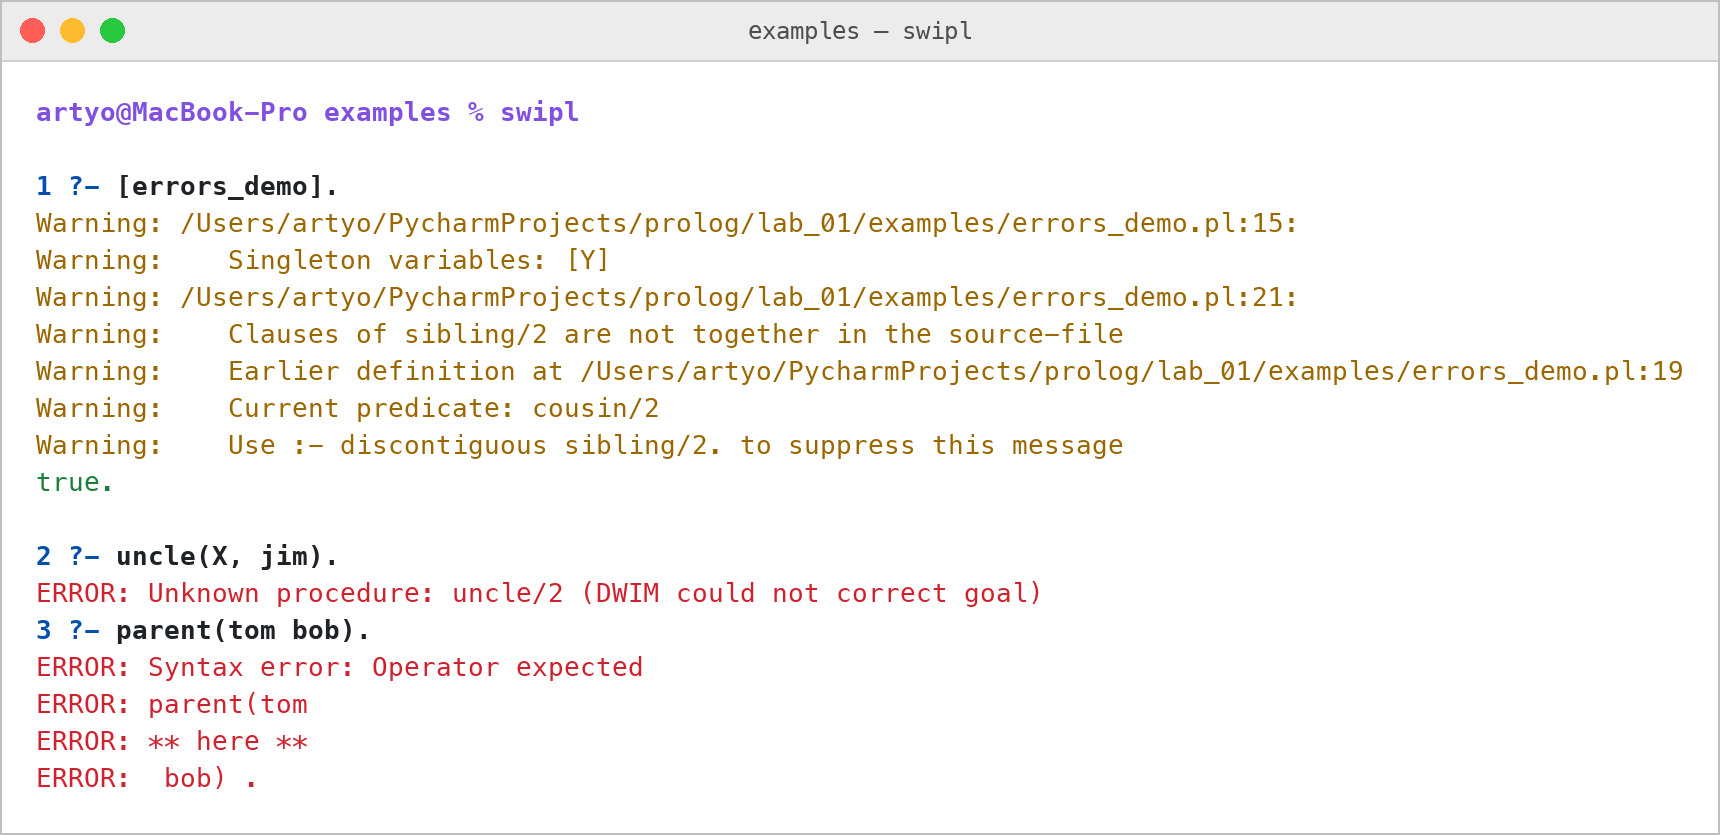
\includegraphics[width=0.95\textwidth]{fig09_errors_a.png}
\caption{Предупреждения при загрузке, неизвестный предикат и синтаксическая ошибка}
\label{fig:errors-a}
\end{figure}

\begin{figure}[H]
\centering
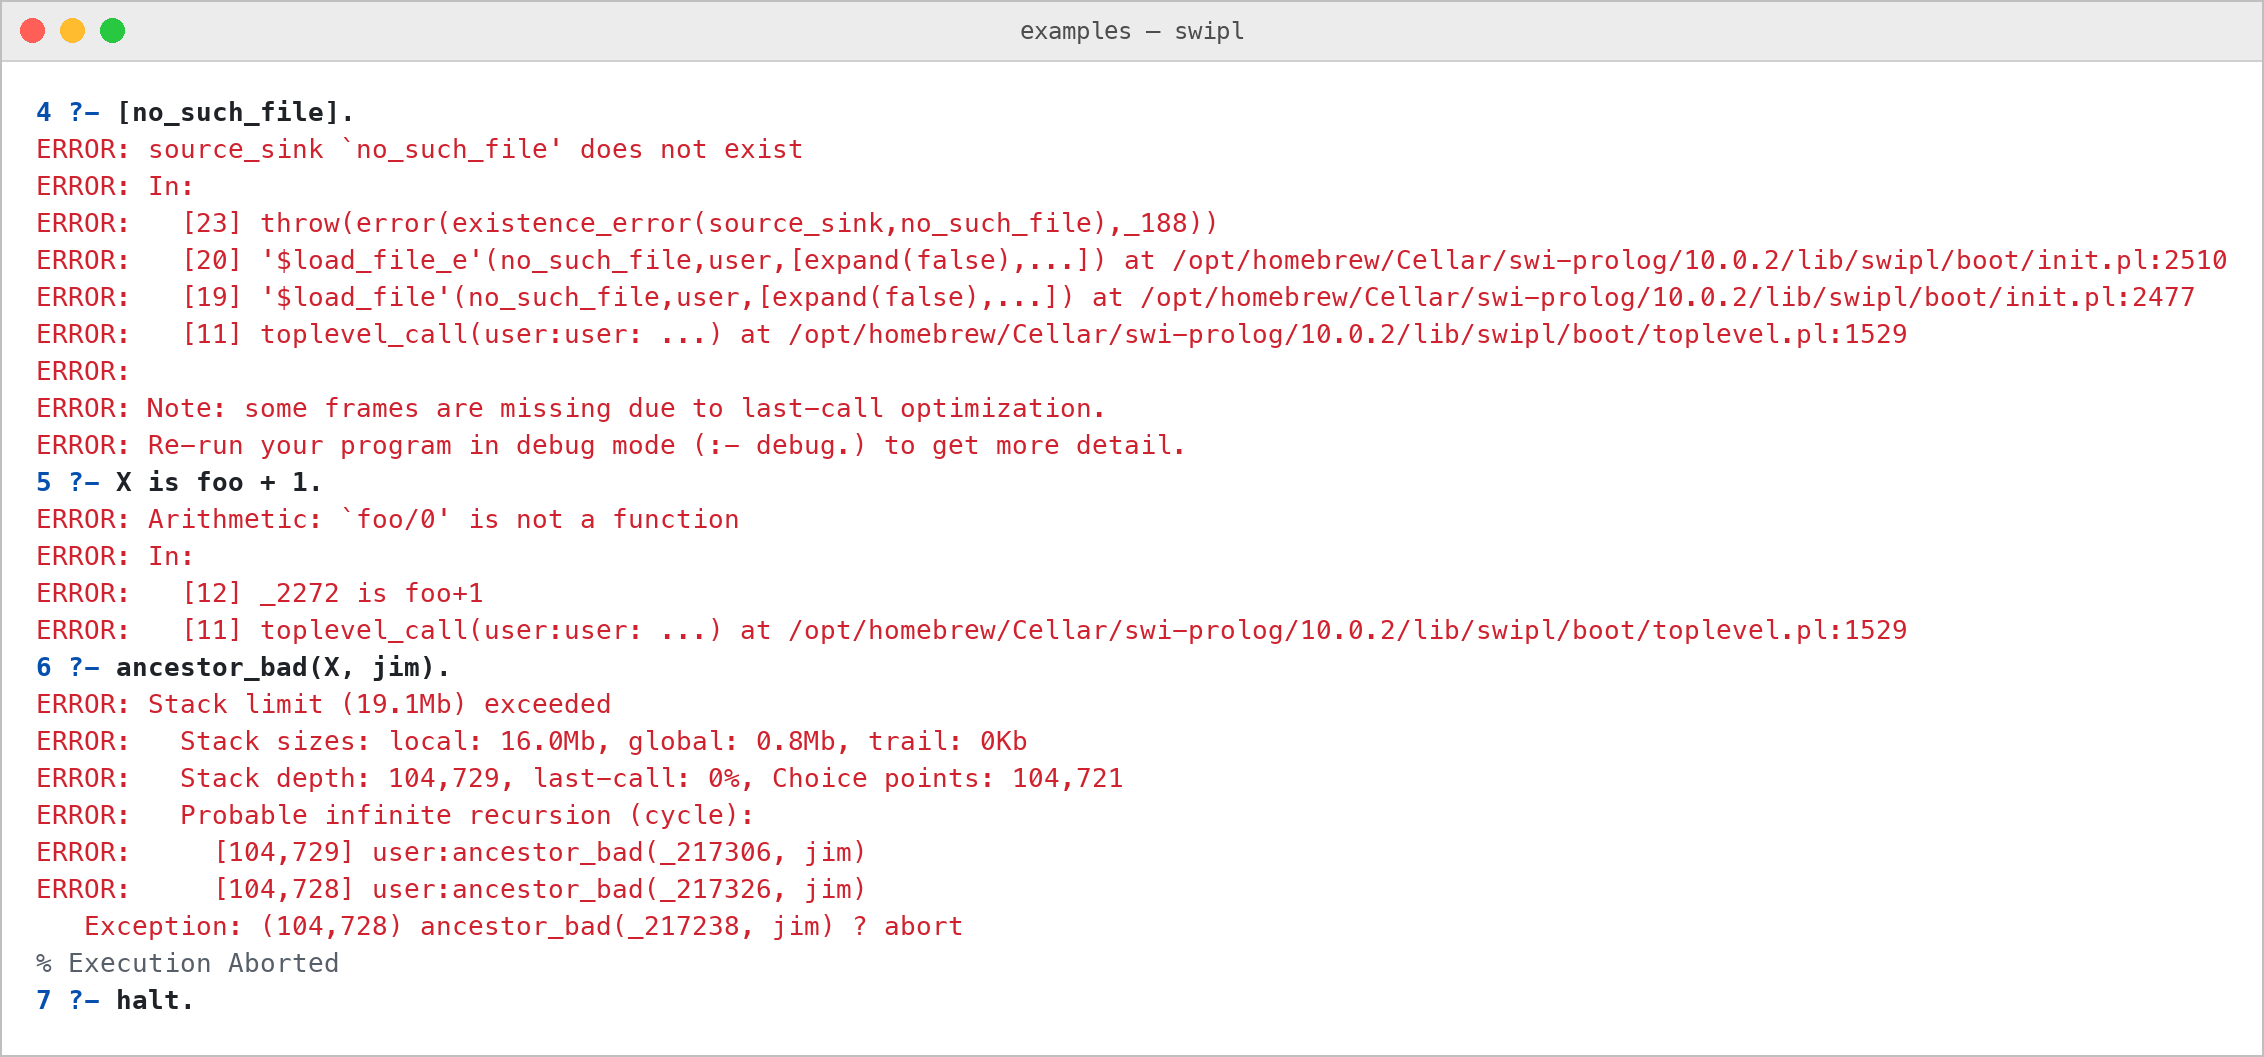
\includegraphics[width=\textwidth]{fig09_errors_b.png}
\caption{Ошибки времени выполнения: отсутствующий файл, арифметика, переполнение стека}
\label{fig:errors-b}
\end{figure}

\begin{enumerate}
\setcounter{enumi}{4}
\item \textbf{Предупреждения при загрузке} не прерывают её (ответ \code{true}), но указывают файл и номер строки. \code{Singleton variables: [Y]} сообщает о переменной, которая встречается в клаузе один раз,~--- обычно это опечатка; \code{Clauses of sibling/2 are not together} сообщает, что определение предиката разорвано другим предикатом, и подсказывает директиву \code{discontiguous} для подавления сообщения.
\item \textbf{Неизвестный предикат.} Запрос к неопределённому \code{uncle/2} приводит не к \code{false}, а к ошибке \code{Unknown procedure}. Механизм DWIM (<<do what I mean>>) пытается найти похожее имя и исправить опечатку; здесь это не удалось.
\item \textbf{Синтаксическая ошибка.} При пропущенной запятой в \code{parent(tom bob)} выводится \code{Operator expected}, а место ошибки отмечается маркером \code{** here **}.
\item \textbf{Отсутствующий файл.} Для \code{[no\_such\_file]} возбуждается исключение \code{existence\_error(source\_sink, \ldots)} с выводом стека вызовов.
\item \textbf{Ошибка типа в арифметике.} В выражении \code{X is foo + 1} атом \code{foo} не является арифметической функцией, о чём сообщается явно.
\item \textbf{Бесконечная рекурсия.} В левой рекурсии \code{ancestor\_bad(X, Y) :- ancestor\_bad(Z, Y), parent(X, Z)} рекурсивный вызов стоит первым и выполняется до проверки фактов, поэтому поиск уходит в бесконечный спуск. SWI-Prolog обнаруживает переполнение стека (для демонстрации предел уменьшен до 20~МБ), указывает на вероятный цикл и переходит в отладчик на порту \code{Exception}, из которого можно выйти командой \code{a} (\code{abort}). Корректное правило \code{ancestor/2} в \code{family.pl} этой проблемы не имеет, так как рекурсивный вызов в нём стоит после \code{parent(X, Z)}.
\end{enumerate}

Сообщения среды информативны: они указывают тип ошибки, файл, строку и предлагают способ исправления. Главное, что нужно усвоить на этом этапе,~--- разница между ответом \code{false} (цель не выводима из базы) и ошибкой (запрос некорректен или предикат не определён).

\section{Выводы}

В ходе работы установлен и настроен SWI-Prolog 10.0.2 под macOS на Apple Silicon, подготовлена рабочая директория для программ, освоены основные команды интерактивной среды: загрузка файлов (\code{consult}, \code{[file]}, \code{make}), просмотр клауз (\code{listing}), справка (\code{help}, \code{apropos}), трассировка (\code{trace}, \code{notrace}, \code{nodebug}) и выход (\code{halt}).

Программа <<Родственные отношения>> загружена и проверена всеми 13 запросами из Приложения~2; полученные ответы совпадают с ожидаемыми. На практике разобраны факты, правила, унификация, рекурсия и возврат, а трассировка показала порядок, в котором Пролог перебирает клаузы и цели.

Серьёзных трудностей не возникло. Единственное расхождение с методическими указаниями~--- дополнительный ответ \code{false} после последнего решения в запросах~9, 10 и~12~--- объясняется тем, что SWI-Prolog сообщает об оставшихся точках выбора. Поведение среды при ошибках изучено на специально подготовленном файле: предупреждения о singleton-переменных и разрывных определениях, ошибки неизвестного предиката, синтаксиса, отсутствующего файла, арифметики и переполнения стека при левой рекурсии.

Результат соответствует поставленной цели: среда логического программирования установлена и настроена, получены навыки работы с top-level, загрузки и выполнения простейших программ.

\newpage
\sectioncenter{Приложение А. Файл для демонстрации диагностики}

Файл \code{lab\_01/examples/errors\_demo.pl} содержит намеренные ошибки: singleton-переменную, разрывное определение предиката и левую рекурсию.

\VerbatimInput{../examples/errors_demo.pl}

\sectioncenter{Приложение Б. Контрольные вопросы для Moodle}

Ниже приведены 30 контрольных вопросов в форме, удобной для визуальной проверки. Исходный банк вопросов для загрузки в Moodle хранится в файле \code{moodle\_questions\_gift.txt} в формате GIFT.

\small
\begin{enumerate}[label=\textbf{\arabic*.}, leftmargin=0pt, itemsep=1.2em]
\item Что в Прологе называется фактом?
\begin{itemize}[label=$\square$, leftmargin=1.5cm, itemsep=0.2em, topsep=0.3em]
\item Клауза с головой и непустым телом, истинная при выполнении условий
\item Клауза без тела, утверждение, истинное безусловно (например, parent(tom, bob).)
\item Вопрос к базе знаний, вводимый после приглашения \texttt{?-}
\item Директива, выполняемая при загрузке файла
\end{itemize}
{\small\textit{Правильный ответ: Клауза без тела, утверждение, истинное безусловно (например, parent(tom, bob).).}}

\item Какая последовательность символов отделяет голову правила от его тела?
\begin{itemize}[label=$\square$, leftmargin=1.5cm, itemsep=0.2em, topsep=0.3em]
\item :-
\item ->
\item :=
\item <-
\end{itemize}
{\small\textit{Правильный ответ: :-.}}

\item Какой запрос загружает файл family.pl в интерактивной среде SWI-Prolog?
\begin{itemize}[label=$\square$, leftmargin=1.5cm, itemsep=0.2em, topsep=0.3em]
\item \texttt{?-} [family].
\item \texttt{?-} load family.
\item \texttt{?-} open(family).
\item \texttt{?-} import(family).
\end{itemize}
{\small\textit{Правильный ответ: \texttt{?-} [family].}}

\item Каким встроенным предикатом завершают работу интерпретатора SWI-Prolog?
\begin{itemize}[label=$\square$, leftmargin=1.5cm, itemsep=0.2em, topsep=0.3em]
\item exit.
\item quit.
\item halt.
\item stop.
\end{itemize}
{\small\textit{Правильный ответ: halt.}}

\item Что ответит SWI-Prolog на запрос \texttt{?-} parent(bob, tom). для программы family.pl?
\begin{itemize}[label=$\square$, leftmargin=1.5cm, itemsep=0.2em, topsep=0.3em]
\item true.
\item false.
\item ERROR: Unknown procedure
\item X = bob.
\end{itemize}
{\small\textit{Правильный ответ: false.}}

\item Какую клавишу нажимают в top-level SWI-Prolog, чтобы получить следующее решение запроса?
\begin{itemize}[label=$\square$, leftmargin=1.5cm, itemsep=0.2em, topsep=0.3em]
\item ; (точка с запятой)
\item Enter
\item . (точка)
\item Esc
\end{itemize}
{\small\textit{Правильный ответ: ; (точка с запятой).}}

\item Как называется механизм возврата к последней точке выбора для поиска альтернативного решения?
\begin{itemize}[label=$\square$, leftmargin=1.5cm, itemsep=0.2em, topsep=0.3em]
\item Унификация
\item Хвостовая рекурсия
\item Возврат (backtracking)
\item Индексация клауз
\end{itemize}
{\small\textit{Правильный ответ: Возврат (backtracking).}}

\item Что такое унификация в Прологе?
\begin{itemize}[label=$\square$, leftmargin=1.5cm, itemsep=0.2em, topsep=0.3em]
\item Объединение двух файлов программы в один
\item Сопоставление двух термов с подбором значений переменных, при которых термы становятся одинаковыми
\item Приведение всех атомов к нижнему регистру
\item Удаление повторяющихся фактов из базы
\end{itemize}
{\small\textit{Правильный ответ: Сопоставление двух термов с подбором значений переменных, при которых термы становятся одинаковыми.}}

\item Какие имена в Прологе обозначают переменные?
\begin{itemize}[label=$\square$, leftmargin=1.5cm, itemsep=0.2em, topsep=0.3em]
\item Имена, начинающиеся со строчной буквы
\item Имена, начинающиеся с заглавной буквы или символа подчёркивания
\item Имена, заключённые в одинарные кавычки
\item Имена, начинающиеся с цифры
\end{itemize}
{\small\textit{Правильный ответ: Имена, начинающиеся с заглавной буквы или символа подчёркивания.}}

\item Чем является tom в факте parent(tom, bob).?
\begin{itemize}[label=$\square$, leftmargin=1.5cm, itemsep=0.2em, topsep=0.3em]
\item Переменной
\item Строкой
\item Атомом (константой)
\item Именем предиката
\end{itemize}
{\small\textit{Правильный ответ: Атомом (константой).}}

\item Какой запрос включает пошаговую трассировку выполнения целей?
\begin{itemize}[label=$\square$, leftmargin=1.5cm, itemsep=0.2em, topsep=0.3em]
\item \texttt{?-} step.
\item \texttt{?-} trace.
\item \texttt{?-} debug\_on.
\item \texttt{?-} verbose.
\end{itemize}
{\small\textit{Правильный ответ: \texttt{?-} trace.}}

\item Какие порты процедурной модели (модели Бёрда) показывает трассировщик SWI-Prolog?
\begin{itemize}[label=$\square$, leftmargin=1.5cm, itemsep=0.2em, topsep=0.3em]
\item Call, Exit, Redo, Fail
\item Start, Stop, Pause, Resume
\item Input, Output, Error, Return
\item Load, Run, Trace, Halt
\end{itemize}
{\small\textit{Правильный ответ: Call, Exit, Redo, Fail.}}

\item Какую роль играет первая клауза ancestor(X, Y) :- parent(X, Y). в определении ancestor/2?
\begin{itemize}[label=$\square$, leftmargin=1.5cm, itemsep=0.2em, topsep=0.3em]
\item Задаёт рекурсивный шаг
\item Задаёт базовый случай рекурсии: родитель является предком
\item Запрещает циклы в родословной
\item Объявляет типы аргументов
\end{itemize}
{\small\textit{Правильный ответ: Задаёт базовый случай рекурсии: родитель является предком.}}

\item Какое первое решение вернёт запрос \texttt{?-} grandparent(X, jim).?
\begin{itemize}[label=$\square$, leftmargin=1.5cm, itemsep=0.2em, topsep=0.3em]
\item X = tom
\item X = bob
\item X = pat
\item false.
\end{itemize}
{\small\textit{Правильный ответ: X = bob.}}

\item Сколько решений имеет запрос \texttt{?-} parent(X, Y). для программы family.pl?
\begin{itemize}[label=$\square$, leftmargin=1.5cm, itemsep=0.2em, topsep=0.3em]
\item 3
\item 4
\item 5
\item 6
\end{itemize}
{\small\textit{Правильный ответ: 5.}}

\item Что означает ответ false. после нескольких нажатий ; в top-level?
\begin{itemize}[label=$\square$, leftmargin=1.5cm, itemsep=0.2em, topsep=0.3em]
\item В программе есть ошибка
\item Найденные ранее решения неверны
\item Других решений нет, перебор исчерпан
\item Запрос содержит синтаксическую ошибку
\end{itemize}
{\small\textit{Правильный ответ: Других решений нет, перебор исчерпан.}}

\item Что делает запрос \texttt{?-} listing(ancestor/2).?
\begin{itemize}[label=$\square$, leftmargin=1.5cm, itemsep=0.2em, topsep=0.3em]
\item Удаляет предикат ancestor/2 из базы
\item Выводит на экран все клаузы предиката ancestor/2
\item Показывает количество решений ancestor/2
\item Включает трассировку ancestor/2
\end{itemize}
{\small\textit{Правильный ответ: Выводит на экран все клаузы предиката ancestor/2.}}

\item Для чего служит запрос \texttt{?-} make.?
\begin{itemize}[label=$\square$, leftmargin=1.5cm, itemsep=0.2em, topsep=0.3em]
\item Компилирует программу в исполняемый файл
\item Перезагружает исходные файлы, изменённые после загрузки
\item Создаёт новый пустой файл программы
\item Собирает проект с помощью утилиты make
\end{itemize}
{\small\textit{Правильный ответ: Перезагружает исходные файлы, изменённые после загрузки.}}

\item Какое сообщение выдаст SWI-Prolog на запрос к неопределённому предикату \texttt{?-} uncle(X, jim).?
\begin{itemize}[label=$\square$, leftmargin=1.5cm, itemsep=0.2em, topsep=0.3em]
\item false.
\item Warning: Singleton variables
\item ERROR: Unknown procedure: uncle/2
\item ERROR: Syntax error: Operator expected
\end{itemize}
{\small\textit{Правильный ответ: ERROR: Unknown procedure: uncle/2.}}

\item О чём предупреждает сообщение Singleton variables: [Y] при загрузке файла?
\begin{itemize}[label=$\square$, leftmargin=1.5cm, itemsep=0.2em, topsep=0.3em]
\item Переменная Y не может быть унифицирована
\item Переменная Y встречается в клаузе только один раз, что часто означает опечатку
\item Переменная Y объявлена глобальной
\item Переменная Y используется в нескольких файлах
\end{itemize}
{\small\textit{Правильный ответ: Переменная Y встречается в клаузе только один раз, что часто означает опечатку.}}

\item Почему правило a(X, Y) :- a(Z, Y), parent(X, Z). приводит к переполнению стека?
\begin{itemize}[label=$\square$, leftmargin=1.5cm, itemsep=0.2em, topsep=0.3em]
\item В теле правила слишком много переменных
\item Это левая рекурсия: рекурсивный вызов стоит первым и выполняется до проверки фактов, поиск уходит в бесконечный спуск
\item Предикат parent/2 не определён
\item SWI-Prolog не поддерживает рекурсию
\end{itemize}
{\small\textit{Правильный ответ: Это левая рекурсия: рекурсивный вызов стоит первым и выполняется до проверки фактов, поиск уходит в бесконечный спуск.}}

\item В каком порядке SWI-Prolog перебирает клаузы предиката и цели в теле правила?
\begin{itemize}[label=$\square$, leftmargin=1.5cm, itemsep=0.2em, topsep=0.3em]
\item Клаузы сверху вниз в порядке записи в файле, цели тела слева направо
\item Клаузы в случайном порядке, цели справа налево
\item Сначала правила, затем факты
\item Клаузы в алфавитном порядке
\end{itemize}
{\small\textit{Правильный ответ: Клаузы сверху вниз в порядке записи в файле, цели тела слева направо.}}

\item Каким запросом можно узнать текущую рабочую директорию в SWI-Prolog?
\begin{itemize}[label=$\square$, leftmargin=1.5cm, itemsep=0.2em, topsep=0.3em]
\item \texttt{?-} current\_dir(D).
\item \texttt{?-} working\_directory(D, D).
\item \texttt{?-} home(D).
\item \texttt{?-} path(D).
\end{itemize}
{\small\textit{Правильный ответ: \texttt{?-} working\_directory(D, D).}}

\item Что вернёт запрос \texttt{?-} findall(X, parent(tom, X), L).?
\begin{itemize}[label=$\square$, leftmargin=1.5cm, itemsep=0.2em, topsep=0.3em]
\item L = bob
\item L = [bob, liz]
\item L = [tom]
\item false.
\end{itemize}
{\small\textit{Правильный ответ: L = [bob, liz].}}

\item Каким запросом открыть встроенную справку по предикату halt/0?
\begin{itemize}[label=$\square$, leftmargin=1.5cm, itemsep=0.2em, topsep=0.3em]
\item \texttt{?-} man(halt).
\item \texttt{?-} info halt.
\item \texttt{?-} help(halt/0).
\item \texttt{?-} doc halt.
\end{itemize}
{\small\textit{Правильный ответ: \texttt{?-} help(halt/0).}}

\item Для чего служит запрос \texttt{?-} apropos(consult).?
\begin{itemize}[label=$\square$, leftmargin=1.5cm, itemsep=0.2em, topsep=0.3em]
\item Загружает файл consult.pl
\item Ищет в документации предикаты и разделы по ключевому слову
\item Выводит исходный код consult/1
\item Отключает предикат consult/1
\end{itemize}
{\small\textit{Правильный ответ: Ищет в документации предикаты и разделы по ключевому слову.}}

\item Какую логическую связку обозначает запятая в теле правила?
\begin{itemize}[label=$\square$, leftmargin=1.5cm, itemsep=0.2em, topsep=0.3em]
\item Конъюнкцию (логическое И)
\item Дизъюнкцию (логическое ИЛИ)
\item Отрицание
\item Импликацию
\end{itemize}
{\small\textit{Правильный ответ: Конъюнкцию (логическое И).}}

\item Какое расширение обычно имеют исходные файлы SWI-Prolog?
\begin{itemize}[label=$\square$, leftmargin=1.5cm, itemsep=0.2em, topsep=0.3em]
\item .swi
\item .pl
\item .prg
\item .lsp
\end{itemize}
{\small\textit{Правильный ответ: .pl.}}

\item Как читается декларативно правило father(X, Y) :- parent(X, Y), male(X).?
\begin{itemize}[label=$\square$, leftmargin=1.5cm, itemsep=0.2em, topsep=0.3em]
\item X — отец Y, если Y — родитель X и Y — мужчина
\item X — отец Y, если X — родитель Y и X — мужчина
\item X — отец Y или X — мужчина
\item Каждый мужчина является отцом
\end{itemize}
{\small\textit{Правильный ответ: X — отец Y, если X — родитель Y и X — мужчина.}}

\item Чем программа на Visual Prolog отличается от программы на SWI-Prolog?
\begin{itemize}[label=$\square$, leftmargin=1.5cm, itemsep=0.2em, topsep=0.3em]
\item В Visual Prolog нет правил, только факты
\item В Visual Prolog обязательны секции domains, predicates и clauses с объявлением типов
\item Visual Prolog не поддерживает рекурсию
\item В Visual Prolog запросы вводятся только в top-level
\end{itemize}
{\small\textit{Правильный ответ: В Visual Prolog обязательны секции domains, predicates и clauses с объявлением типов.}}
\end{enumerate}
\normalsize


\end{document}
